%% 独立编译测试用主文件（xelatex 编译）
\documentclass[12pt,a4paper]{ctexart}

\usepackage{amsmath,amssymb,amsthm}
\usepackage{booktabs}
\usepackage{graphicx}
\usepackage{geometry}
\usepackage{caption}
\usepackage{algorithm}
\usepackage{algpseudocode}
\usepackage{xcolor}

\geometry{left=2.5cm,right=2.5cm,top=2.5cm,bottom=2.5cm}

\newtheorem{remark}{注}
\floatname{algorithm}{算法}
\renewcommand{\algorithmicrequire}{\textbf{输入:}}
\renewcommand{\algorithmicensure}{\textbf{输出:}}

\title{2026 年中国研究生数学建模竞赛 D 题\\
       山区洪涝灾害下无人机运输与通信协同优化}
\author{}
\date{}

\begin{document}
\maketitle

%% ===================================================================
%%  2026 年中国研究生数学建模竞赛  D 题
%%  第二问：多机协同调度与三维理论边界分析
%%  编译方式：xelatex（需中文支持）
%% ===================================================================

\section{问题二：多机协同调度与三维理论边界分析}

\subsection{问题分析}

问题二在问题一单点往返的基础上同时放开三项限制：允许\textbf{跨服务区组批}，
即一个架次可依次访问多个服务区；引入\textbf{实体无人机数量}与\textbf{共享电池库存}；
并要求满足\textbf{配送时限}。三项限制耦合后，问题不再能像问题一那样分解为
$15$ 个独立子问题，而成为一个同时包含"选架次"与"排时序"两层决策的优化问题。

记调度中心为 $O_{01}$，服务区集合 $\mathcal{S}=\{S_{001},\dots,S_{015}\}$，
货箱集合 $\mathcal{B}$（$|\mathcal{B}|=80$）。资源配置见表~\ref{tab:q2-res}。

\begin{table}[htbp]
  \centering
  \caption{无人机与电池资源配置}
  \label{tab:q2-res}
  \begin{tabular}{ccccccc}
    \toprule
    机型 $g$ & 整机数 $K_g$ & 电池组数 $B_g$ & 载重 $Q_g$/kg
      & 舱容 $V_g$/m$^3$ & 可用电量 $E_g^{\mathrm{use}}$/kWh
      & 满充时间 $T_g^{\mathrm{chg}}$/s \\
    \midrule
    A & 4 & 6 & 25 & 0.060 & 4.5 & 1800 \\
    B & 2 & 4 & 30 & 0.073 & 4.0 & 2400 \\
    C & 2 & 4 & 80 & 0.250 & 8.0 & 3000 \\
    \midrule
    合计 & \textbf{8} & \textbf{14} & --- & --- & --- & --- \\
    \bottomrule
  \end{tabular}
\end{table}

本问的关键建模细节在于\textbf{区分两类资源的占用区间}。设架次 $j$ 于时刻 $s_j$
出发、飞行时长为 $d_j$、返航后需充电 $c_j$，则

\begin{equation}
  \underbrace{[\,s_j,\;s_j+d_j\,)}_{\text{整机占用}},
  \qquad
  \underbrace{[\,s_j,\;s_j+d_j+c_j\,)}_{\text{电池占用}} .
\end{equation}

电池占用区间比整机长 $c_j$。由于 C 型满充需 $3000$~s，远超其典型飞行时长，
故\textbf{电池而非整机}往往构成真正的系统瓶颈——这一判断将在第
\ref{subsec:q2-bottleneck} 节得到定量印证。若建模时遗漏充电段而仅以
$[s_j,s_j+d_j)$ 约束电池，将得到偏乐观且不可实施的调度方案。

优化目标为在保证时效性前提下最小化\textbf{完工时刻}
\begin{equation}
  C_{\max}=\max_{j\in\mathcal{J}}\,\bigl(s_j+d_j\bigr),
\end{equation}
其中 $\mathcal{J}$ 为被选中的架次集合。

\subsection{模型建立}

\subsubsection{决策变量}

设候选架次池为 $\mathcal{P}$（生成方式见第 \ref{subsec:q2-pool} 节），
对每个候选 $j\in\mathcal{P}$ 引入

\begin{equation}
  x_j\in\{0,1\}:\ \text{是否选用候选 } j,
  \qquad
  s_j\in\mathbb{Z}_{\ge 0}:\ \text{其出发时刻} .
\end{equation}

记 $\mathcal{B}_j$ 为候选 $j$ 承运的货箱集合，$g(j)$ 为其机型，
$\mathcal{P}_g=\{j\in\mathcal{P}\mid g(j)=g\}$。

\subsubsection{约束条件}

\textbf{（1）货箱分划约束。} 每个货箱恰好被交付一次，不重不漏：
\begin{equation}
  \sum_{j\in\mathcal{P}:\,b\in\mathcal{B}_j} x_j = 1,
  \qquad \forall\,b\in\mathcal{B} .
  \label{eq:q2-cover}
\end{equation}

\textbf{（2）架次数约束。} 用于绘制 $N$--$C_{\max}$ 权衡曲线：
\begin{equation}
  \sum_{j\in\mathcal{P}} x_j = N .
\end{equation}

\textbf{（3）整机与电池资源约束。} 对每个机型 $g$ 施加累积型（cumulative）约束，
保证任意时刻并发占用不超过资源上限：
\begin{align}
  \sum_{j\in\mathcal{P}_g}\mathbf{1}\!\left[t\in[s_j,\,s_j+d_j)\right]x_j
    &\le K_g, &&\forall\,t\ge 0,\ \forall\,g, \\
  \sum_{j\in\mathcal{P}_g}\mathbf{1}\!\left[t\in[s_j,\,s_j+d_j+c_j)\right]x_j
    &\le B_g, &&\forall\,t\ge 0,\ \forall\,g .
  \label{eq:q2-cumul}
\end{align}

\textbf{（4）时效性约束。} 记货箱 $b$ 在架次 $j$ 内的交付偏移为 $o_{jb}$，
期望送达时刻 $T_b^{\mathrm{exp}}$，硬截止时刻 $T_b^{\mathrm{dead}}$：
\begin{equation}
  s_j+o_{jb}\le T_b^{\mathrm{exp}},
  \qquad
  s_j+o_{jb}\le T_b^{\mathrm{dead}},
  \qquad \forall\,j\in\mathcal{P},\ \forall\,b\in\mathcal{B}_j .
  \label{eq:q2-time}
\end{equation}

本文采用\textbf{严格时效}口径，即要求全部 $80$ 箱均不晚于期望送达时刻
（加权延误为零）。该口径严格强于"仅满足硬截止"的宽松口径，后者会显著低估
$C_{\max}$，两者所得数值不具可比性。

\textbf{（5）容量与电量约束。}
\begin{equation}
  \sum_{b\in\mathcal{B}_j} m_b \le Q_{g(j)},
  \qquad
  \sum_{b\in\mathcal{B}_j} v_b \le V_{g(j)},
  \qquad
  E_j \le (1-\rho)\,E^{\mathrm{use}}_{g(j)},
\end{equation}
其中 $\rho=0.20$ 为返航安全余量，沿用问题一口径。

\subsubsection{实体无人机与电池的指派}
\label{subsec:q2-color}

题目要求"联合确定\ldots\ 具体执行无人机、共享电池"。
注意到累积约束 \eqref{eq:q2-cumul} 仅保证任意时刻并发占用不超过资源上限，
而未显式指定每个架次由哪一台实体设备执行。事实上二者是等价的——
由 Dilworth 定理的区间图特例可知，区间图的最小染色数等于其最大团数，
而区间图的最大团恰为某时刻的最大并发数。因此

\begin{equation}
  \text{式 \eqref{eq:q2-cumul} 成立}
  \iff
  \exists\ \text{一组合法的实体指派},
\end{equation}

即满足累积约束的调度\textbf{必然存在}可行的实体分配方案。

据此，本文在求解完成后采用\textbf{区间图贪心着色}构造实体指派：
将各架次按开始时刻升序排列，维护一个空闲设备池；处理架次 $j$ 时，
先将所有已于 $s_j$ 前释放的设备回收至空闲池，再从中取出编号最小者分配给 $j$。
对整机按区间 $[s_j,s_j+d_j)$ 着色，对电池按 $[s_j,s_j+d_j+c_j)$ 着色。
该过程对每个机型独立执行，时间复杂度 $O(n\log n)$。

由上述等价性，着色必然成功且所用设备数不超过 $K_g$（或 $B_g$）；
若着色过程中出现空闲池为空，则反证原调度违反累积约束，可作为
\textbf{独立于求解器的校验手段}——这正是第 \ref{subsec:q2-verify} 节
验证程序的核心机制。

\subsubsection{完整模型}

综上，问题二的混合整数规划模型为
\begin{equation}
  \begin{aligned}
    \min\quad & C_{\max}=\max_{j:\,x_j=1}\,(s_j+d_j) \\
    \mathrm{s.t.}\quad
      & \text{式 \eqref{eq:q2-cover}--\eqref{eq:q2-time}}, \\
      & x_j\in\{0,1\},\quad s_j\in\mathbb{Z}_{\ge 0},
        \qquad \forall\,j\in\mathcal{P} .
  \end{aligned}
  \label{eq:q2-model}
\end{equation}

\subsection{候选架次池的生成与物理模型校准}
\label{subsec:q2-pool}

候选池沿用问题一冻结的统一物理模型。为保证数值可复现，对三个易错常数
做了反解校准，见表~\ref{tab:q2-calib}。

\begin{table}[htbp]
  \centering
  \caption{物理模型常数校准}
  \label{tab:q2-calib}
  \begin{tabular}{lll}
    \toprule
    常数 & 取值 & 说明 \\
    \midrule
    $R_{\mathrm{earth}}$ & $6\,378\,137.0$~m
      & WGS-84 长半轴（非平均半径 $6\,371\,000$~m）；\\
    & & 由 $300$ 条航段反解，标准差 $<10^{-6}$ \\
    $g$ & $9.81$~m/s$^2$
      & 取 $9.8$ 会使爬升能耗整体偏 $1.00102$ 倍 \\
    DEM 采样步长 & $1.0$~m
      & 步长 $15$~m 时个别航段巡航高度偏差达 $10.14$~m，需 $\le 3$~m \\
    \bottomrule
  \end{tabular}
\end{table}

校准后对基准池全部 $572$ 个候选逐条复算，\textbf{时长误差 $0.000\,000\,00$~s、
能耗误差 $0.000\,000\,000\,0$~kWh、航段字段最大偏差 $1.1\times 10^{-9}$}，
可认为与基准完全一致。在此基础上枚举跨区组批与访问顺序，经支配剪枝
（同机型、同货箱集合下仅保留时长最短的路线）后得到规模 $11\,936$ 的候选池。

\subsection{三类理论下界}
\label{subsec:q2-bounds}

为评估解的质量并提供与算法无关的性能基准，本文推导三个下界。
\textbf{三者均仅依赖必要条件，任何可行解都必须满足，故均为严格下界。}
三类下界的松弛思路与紧致程度汇总于第 \ref{subsec:q2-bounds} 节末尾。

\subsubsection{架次数下界：装箱松弛}

松弛掉"同一架次的货箱须同属一条可行航线"这一耦合，问题退化为装箱
（bin packing）问题。按最大机型 C（$Q=80$~kg，$V=0.25$~m$^3$）计算连续松弛：
\begin{equation}
  N_{\mathrm{lb}}\ \ge\
  \max\left\{
    \left\lceil \frac{\sum_b m_b}{\max_g Q_g}\right\rceil,\
    \left\lceil \frac{\sum_b v_b}{\max_g V_g}\right\rceil
  \right\}
  =\max\left\{
    \left\lceil \frac{758.00}{80}\right\rceil,\
    \left\lceil \frac{2.0110}{0.25}\right\rceil
  \right\}
  =\max\{10,\,9\}=10 .
\end{equation}

进一步以 CP-SAT 求解\textbf{不劈箱}的精确装箱模型（同时施加载重与舱容约束，
并以 $y_k\ge y_{k+1}$ 破除对称性），求得下界同为 $10$，求解状态为 OPTIMAL。故
\begin{equation}
  \boxed{\,N_{\mathrm{lb}}=10\,}
\end{equation}

\subsubsection{完工时刻下界：聚合面积松弛}

松弛掉逐架次的时序排布，仅保留"资源总供给不小于总需求"这一必要条件。
在时间窗 $[0,C_{\max}]$ 内，机型 $g$ 的 $K_g$ 台整机至多提供 $K_g C_{\max}$
机时，$B_g$ 组电池至多提供 $B_g C_{\max}$ 池时，于是
\begin{equation}
  \sum_{j\in\mathcal{P}_g} d_j\,x_j \;\le\; K_g\,C_{\max},
  \qquad
  \sum_{j\in\mathcal{P}_g} (d_j+c_j)\,x_j \;\le\; B_g\,C_{\max},
  \qquad \forall\,g\in\{A,B,C\} .
  \label{eq:q2-area}
\end{equation}

式 \eqref{eq:q2-area} 是式 \eqref{eq:q2-cumul} 在时间轴上的积分，
因而是后者的必要条件。该松弛模型不含 $s_j$ 变量与累积约束，
仅为 $0$--$1$ 选择加线性面积约束，在万级候选池上可秒级求得 OPTIMAL：
\begin{equation}
  \boxed{\,C_{\max}^{\mathrm{lb}}=5942~\mathrm{s}\,}
  \qquad (N=23\ \text{固定，严格时效})
\end{equation}

若放开架次数限制，下界降至 $5604$~s（对应 $N=26$）。

\begin{remark}
$5942$~s 是"面积可容纳"意义下的下界，\textbf{并不等于可达}。
在后续实验中，该配比下的多个架次组合均被证明时序不可排（INFEASIBLE），
说明"资源总量够"与"时序排得开"是两个不同的命题，真实最优值严格高于此值。
该下界的作用是提供不可达性判据，而非可达性保证。
\end{remark}

\subsubsection{总能耗下界：集合分划松弛}

丢弃全部时间与资源约束，仅保留货箱分划约束 \eqref{eq:q2-cover}，
最小化总能耗：
\begin{equation}
  E_{\mathrm{lb}}=\min\left\{
    \sum_{j\in\mathcal{P}} E_j x_j
    \ \middle|\
    \sum_{j:\,b\in\mathcal{B}_j} x_j=1,\ \forall b\in\mathcal{B}
  \right\}.
\end{equation}

求解结果（均为 OPTIMAL）：
\begin{equation}
  E_{\mathrm{lb}}^{\,\mathrm{free}}=59.7145~\mathrm{kWh}\ (N=19),
  \qquad
  \boxed{\,E_{\mathrm{lb}}^{\,N=23}=60.4415~\mathrm{kWh}\,}
\end{equation}

值得注意的是，$E_{\mathrm{lb}}$ 随 $N$ 增大而\textbf{上升}——架次越多，
固定起降能耗摊销次数越多。故能耗下界必须在同一 $N$ 下比较，
跨 $N$ 比较无意义。

\subsubsection{下界汇总与解质量评估}

三类下界与本文解的对比见表~\ref{tab:q2-bounds} 与图~\ref{fig:q2-bounds}。

\begin{table}[htbp]
  \centering
  \caption{三类理论下界与本文解的对比}
  \label{tab:q2-bounds}
  \begin{tabular}{lcccc}
    \toprule
    指标 & 理论下界 & 本文解 (bd23) & 绝对缺口 & 相对缺口 \\
    \midrule
    架次数 $N$            & 10      & 23       & 13      & --- \\
    完工时刻 $C_{\max}$/s & 5942    & \textbf{6568.17} & 626.83 & 10.5\,\% \\
    总能耗 $E$/kWh        & 60.4415 & 71.3885  & 10.9470 & 18.1\,\% \\
    \bottomrule
  \end{tabular}
\end{table}

\begin{figure}[htbp]
  \centering
  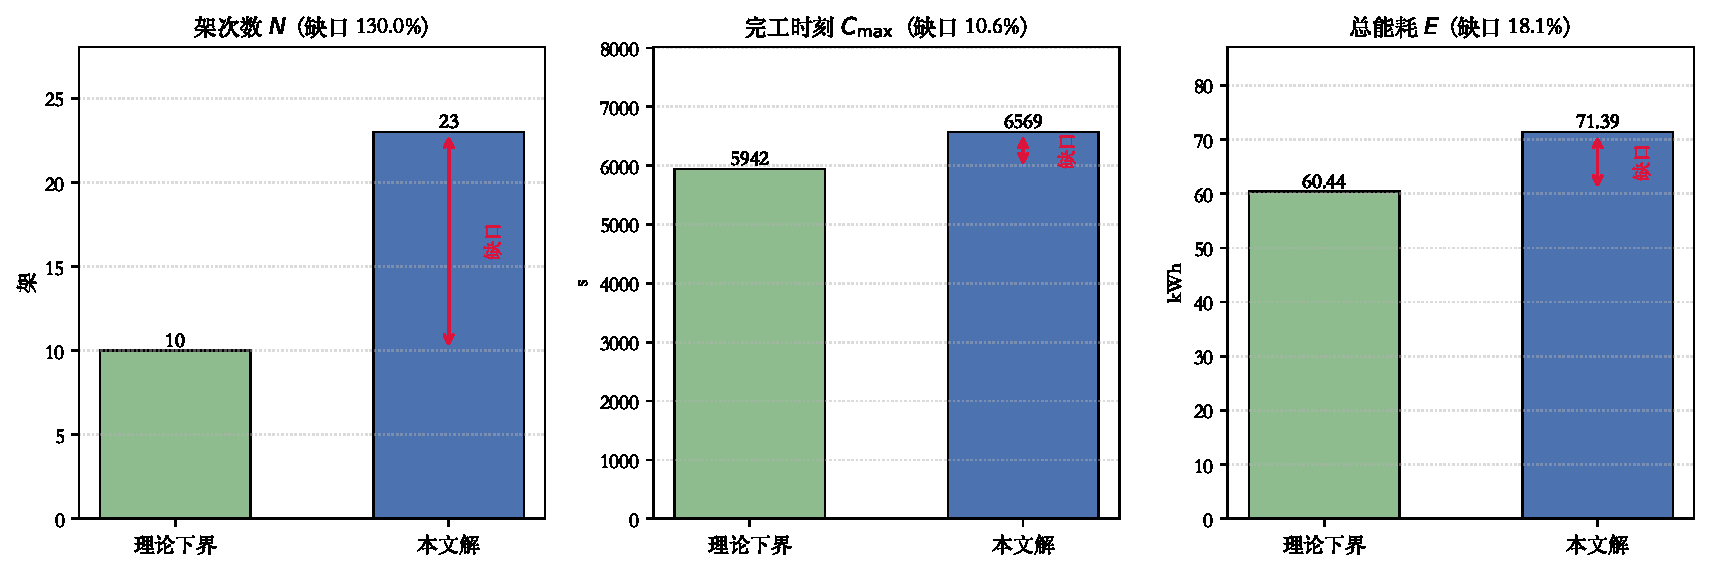
\includegraphics[width=0.95\textwidth]{图/q2_fig2_bounds.pdf}
  \caption{三类理论下界与本文解的对比}
  \label{fig:q2-bounds}
\end{figure}

三个下界的紧致程度差异显著，须分别解读，不可一概而论。

$N_{\mathrm{lb}}=10$ \textbf{极为宽松}。它完全忽略了时效性与航程约束——
事实上 $10$ 个架次无论如何排布都不可能在期望时限内覆盖 $15$ 个分散服务区。
该下界的意义仅在于刻画容量刚性底线，\textbf{不应被解读为"尚有 13 架次的
优化空间"}。

$C_{\max}^{\mathrm{lb}}=5942$~s \textbf{相对最紧}（缺口 $10.5\,\%$），
因为面积松弛已捕获本问的主导矛盾——资源总量与时间窗之比。

$E_{\mathrm{lb}}$ 的缺口主要源于：能耗最优的架次组合（$19$ 架次）与
时效最优的组合（$23$ 架次）并不重合，为满足严格时效必须牺牲部分能耗。

\subsection{瓶颈诊断与求解策略}
\label{subsec:q2-bottleneck}

\subsubsection{瓶颈定位}

对中间解（$C_{\max}=6875$~s，配比 A$=$10/B$=$6/C$=$7）做负载分解，
结果见表~\ref{tab:q2-diag}。

\begin{table}[htbp]
  \centering
  \caption{中间解的机型负载分解（暴露 C 型电池瓶颈）}
  \label{tab:q2-diag}
  \begin{tabular}{ccccc}
    \toprule
    机型 & 架次数 & 飞行总时长/机队 & (飞行$+$充电)/电池 & 瓶颈 \\
    \midrule
    A & 10 & $20823/4=5206$~s & $32534/6=5422$~s & \\
    B & 6  & $12027/2=6014$~s & $22749/4=5687$~s & \\
    C & 7  & $13328/2=6664$~s & $\mathbf{27195/4=6799}$~s & $\leftarrow$ \\
    \bottomrule
  \end{tabular}
\end{table}

C 型在 $7$ 架次时\textbf{电池负载 $6799$~s 超过整机负载 $6664$~s}，
直接顶住 $C_{\max}$。这印证了第 2.1 节的判断：C 型满充 $3000$~s，
$4$ 组电池支撑 $7$ 个架次时周转不过来。

\subsubsection{破局方向}

面积松弛给出的最优配比为 \textbf{A$=$10 / B$=$7 / C$=$6}，
三机型负载被压平至 $5794/5916/5940$~s。关键在于将 C 型从 $7$ 架次降至
$6$ 架次——仅移动一个架次，即可解除电池瓶颈。

据此本文曾尝试"为 C 型筛选低能耗架次以加快电池周转"（能耗低
$\Rightarrow$ 充电快），构造了 C 型充电时间 $683$--$2534$~s 的专用候选池，
但仅将 $C_{\max}$ 从 $6875$~s 降至 $6857$~s，且在 $6287$~s 处判定不可行。
该实验表明：\textbf{正确方向不是让 C 型飞得更省，而是让它少飞一个架次。}

\subsubsection{逻辑型 Benders 分解}

直接将"选架次"与"排时序"合并为单一 CP-SAT 模型时，
在 $2329$ / $5797$ / $11\,936$ / $21\,547$ 四种池规模下\textbf{均返回 UNKNOWN}，
即便给定 $900$~s 预算也无法找到首个可行解——累积约束叠加数千个可选区间
使约束传播机制失效。

为此采用逻辑型 Benders 分解，将式 \eqref{eq:q2-model} 拆为两层：

\begin{itemize}
  \item \textbf{主问题（Master）}：仅含 $0$--$1$ 选择与面积约束
        \eqref{eq:q2-area}，秒级求得 OPTIMAL。其目标值恒为真实 $C_{\max}$
        的下界；
  \item \textbf{子问题（Sub）}：固定主问题选出的 $N$ 个架次，
        仅对这 $N$ 个区间排时序，规模极小，秒级可解；
  \item \textbf{割（Cut）}：若子问题不可行，向主问题追加
        $\sum_{j\in S} x_j\le |S|-1$，排除该组合后重解。
\end{itemize}

该框架的核心优点是\textbf{主问题目标值天然提供下界}，
故算法输出的 $[\mathrm{LB},\mathrm{UB}]$ 区间是带证明的，
而非启发式的经验值。完整流程见算法~\ref{alg:q2-benders}。

\begin{algorithm}[htbp]
  \caption{逻辑型 Benders 分解求解 $\min C_{\max}$}
  \label{alg:q2-benders}
  \begin{algorithmic}[1]
    \State 初始化 $\mathrm{UB}\gets$ 已知可行解, $\mathrm{LB}\gets 0$
    \For{$\mathrm{iter}=1,2,\dots$}
      \State 求解主问题，得架次集合 $S$ 与松弛值 $z$
      \State $\mathrm{LB}\gets\max(\mathrm{LB},\,z)$
      \State 固定 $S$ 求解子问题，得真实 $C_{\max}(S)$
      \If{子问题可行 \textbf{且} $C_{\max}(S)<\mathrm{UB}$}
        \State $\mathrm{UB}\gets C_{\max}(S)$；记录当前解
      \EndIf
      \State 向主问题追加割 $\sum_{j\in S}x_j\le|S|-1$
      \If{$\mathrm{UB}-\mathrm{LB}\le\varepsilon$}
        \State \textbf{break}
      \EndIf
    \EndFor
    \State \Return 最优解及区间 $[\mathrm{LB},\mathrm{UB}]$
  \end{algorithmic}
\end{algorithm}

\subsection{求解结果与分析}

\subsubsection{最优调度方案}

最优解 bd23 的关键指标见表~\ref{tab:q2-result}。

\begin{table}[htbp]
  \centering
  \caption{最优解 bd23 的关键指标}
  \label{tab:q2-result}
  \begin{tabular}{ll}
    \toprule
    项目 & 数值 \\
    \midrule
    架次数 $N$              & 23 \\
    \textbf{完工时刻 $C_{\max}$} & \textbf{6568.168~s} \\
    总能耗                  & 71.3885~kWh \\
    机型配比                & A$=$10 / B$=$7 / C$=$6 \\
    按期交付                & \textbf{80/80}（加权延误 $0$） \\
    硬截止                  & 31 箱全部满足，最小余量 277.686~s \\
    资源占用                & 整机 8/8，电池 14/14 \\
    最小电量余量            & 0.010886~kWh \\
    \bottomrule
  \end{tabular}
\end{table}

完整调度甘特图见图~\ref{fig:q2-gantt}。图 (a) 为整机占用，
图 (b) 为电池占用（含充电段）。可以直观看到：电池的斜纹充电段显著长于
飞行段，尤其 C 型电池在整个时间窗内几乎满负荷周转，
与第 \ref{subsec:q2-bottleneck} 节的瓶颈诊断一致。

\begin{figure}[htbp]
  \centering
  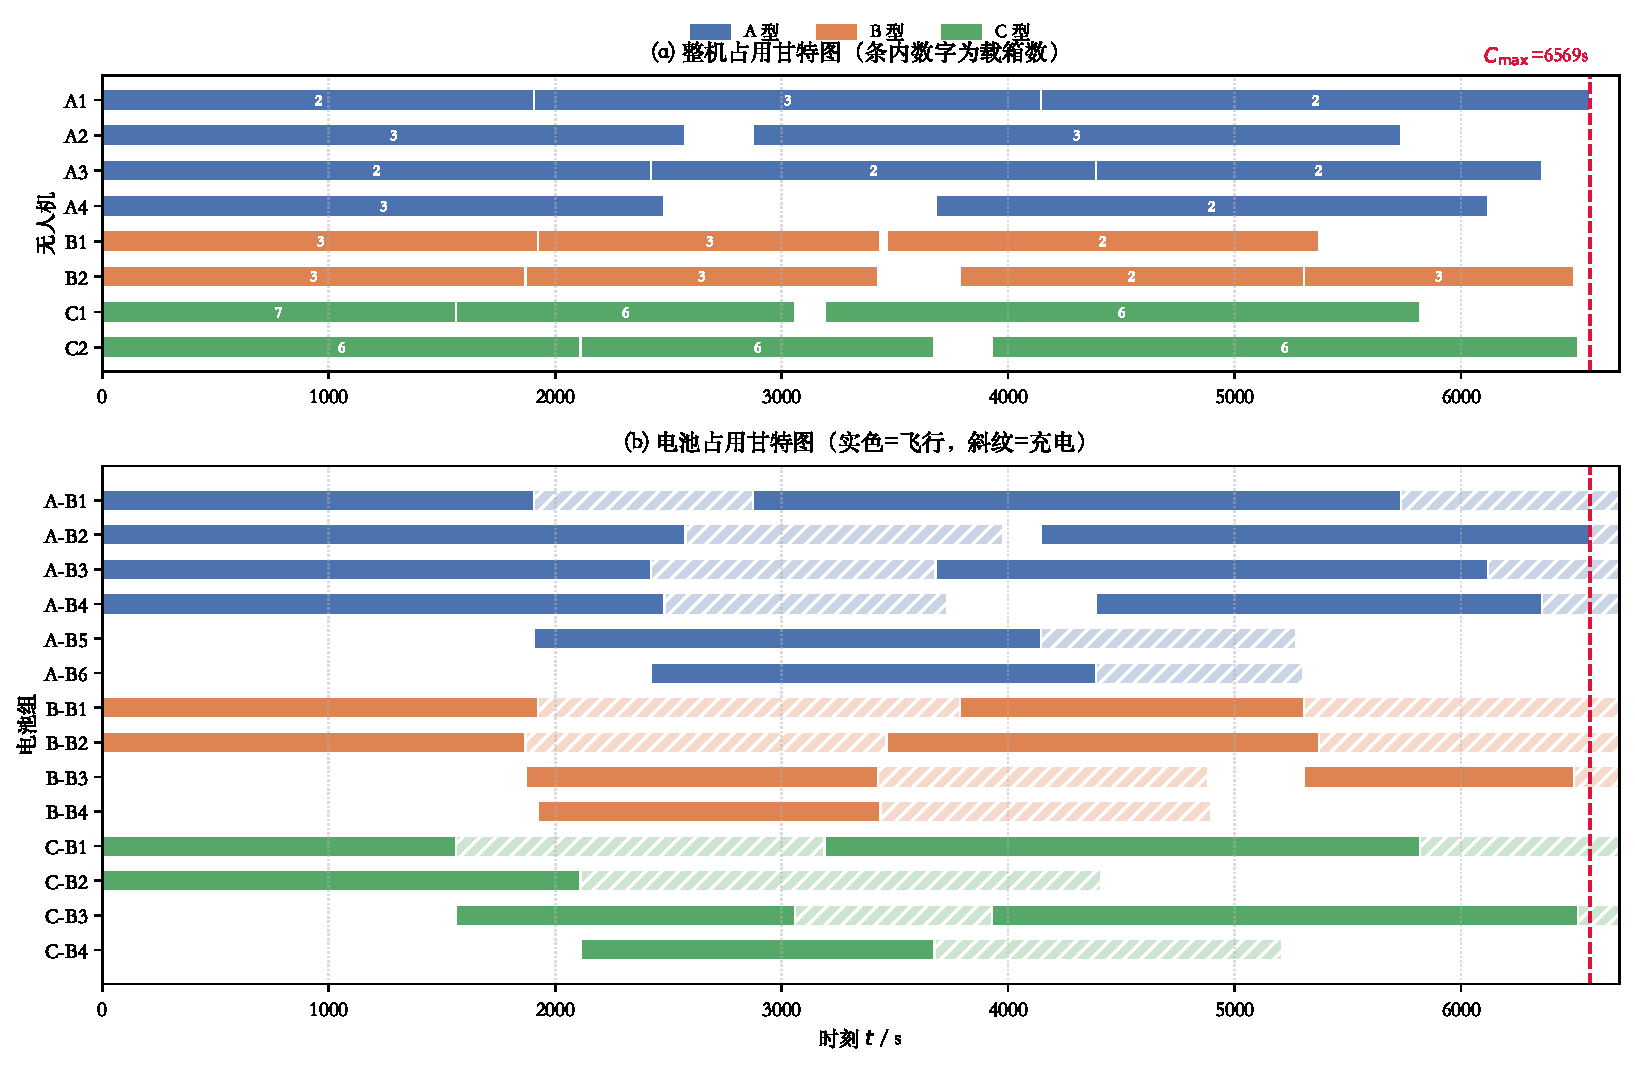
\includegraphics[width=\textwidth]{图/q2_fig1_gantt.pdf}
  \caption{最优解 bd23 的整机与电池占用甘特图}
  \label{fig:q2-gantt}
\end{figure}

\subsubsection{负载均衡性分析}

各机型负载分解见表~\ref{tab:q2-load} 与图~\ref{fig:q2-load}。

\begin{table}[htbp]
  \centering
  \caption{最优解 bd23 的机型负载分解}
  \label{tab:q2-load}
  \begin{tabular}{cccc}
    \toprule
    机型 & 架次数 & 飞行/机队 & (飞行$+$充电)/电池 \\
    \midrule
    A & 10 & $23283/4=5821$~s & $35237/6=5873$~s \\
    B & 7  & $11478/2=5739$~s & $22594/4=5648$~s \\
    C & 6  & $11947/2=5973$~s & $23021/4=5755$~s \\
    \bottomrule
  \end{tabular}
\end{table}

\begin{figure}[htbp]
  \centering
  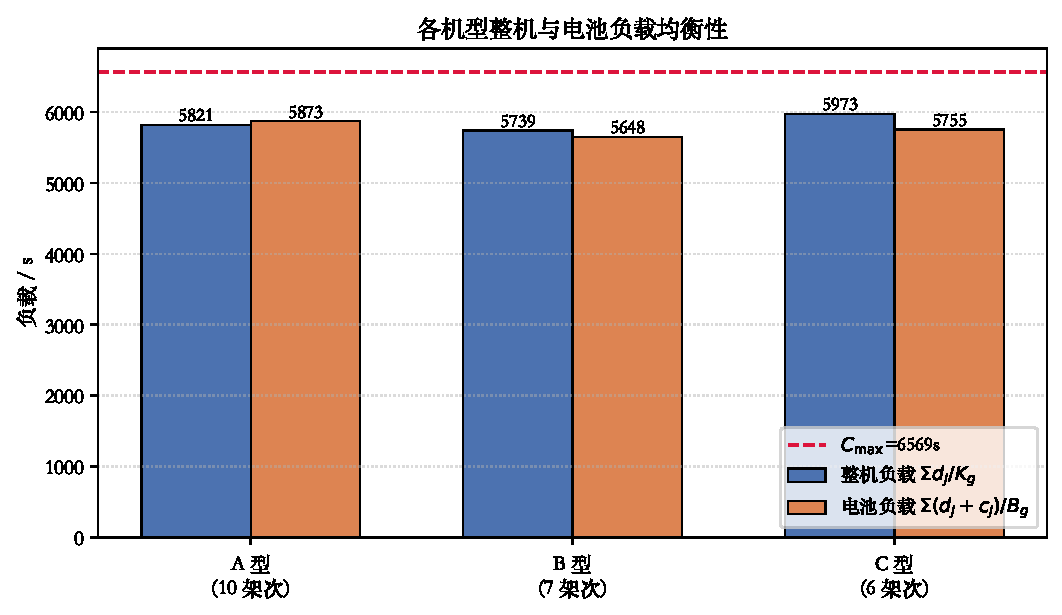
\includegraphics[width=0.8\textwidth]{图/q2_fig4_load.pdf}
  \caption{各机型整机与电池负载均衡性}
  \label{fig:q2-load}
\end{figure}

三机型整机负载分别为 $5821/5739/5973$~s，\textbf{极差仅 $234$~s}，
表明资源配置已高度均衡，印证了第 \ref{subsec:q2-bottleneck} 节
关于配比的判断。$C_{\max}=6568$~s 与最大负载 $5973$~s 之间的
$595$~s 差额，源于时效性约束 \eqref{eq:q2-time} 导致的不可避免的等待窗口：
部分服务区的期望送达时刻较早，迫使相关架次必须在特定时段出发，
无法完全填满资源空档。

\subsubsection{四项指标的权衡关系}

题目要求综合考虑\textbf{配送及时性、全部任务完成时间、运输能耗、架次数}
四项指标并说明其权衡关系。四者的两两关系如图~\ref{fig:q2-tradeoff} 所示。

\begin{figure}[htbp]
  \centering
  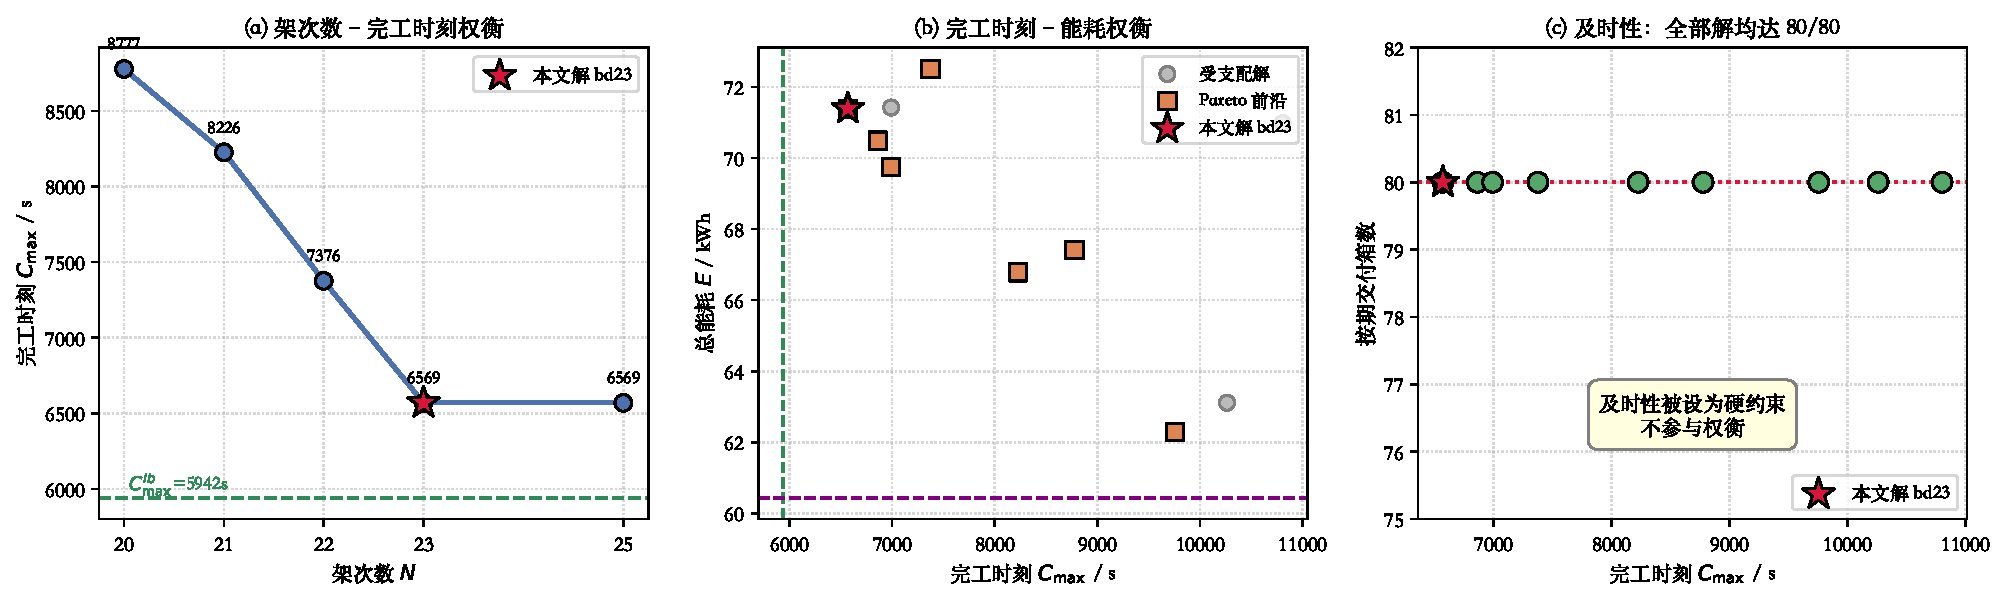
\includegraphics[width=\textwidth]{图/q2_fig5_tradeoff.pdf}
  \caption{四项指标的权衡关系}
  \label{fig:q2-tradeoff}
\end{figure}

\paragraph{（1）架次数 $N$ 与完工时刻 $C_{\max}$：先强替代、后饱和。}
由图~\ref{fig:q2-tradeoff}(a)，随 $N$ 由 $20$ 增至 $23$，
$C_{\max}$ 由 $8777$~s 单调降至 $6569$~s，降幅达 $25.2\,\%$。
其机理在于：架次数越多，单架次载荷越小、飞行时长越短，
从而更易填充资源空档、提升并行度。但该替代关系在 $N=23$ 处\textbf{饱和}——
继续增至 $N=25$ 时 $C_{\max}$ 不再下降（仍为 $6569$~s），
因为此时瓶颈已由"架次不足"转为"电池周转能力"（见第
\ref{subsec:q2-bottleneck} 节），增加架次反而加剧电池争用。
故 $N=23$ 是该权衡曲线的\textbf{拐点}，这也是本文选定 $N=23$ 的依据。

\paragraph{（2）完工时刻 $C_{\max}$ 与能耗 $E$：显著互斥。}
由图~\ref{fig:q2-tradeoff}(b)，能耗最优解 eN22（$62.29$~kWh）
对应 $C_{\max}=9757$~s，比 bd23 慢 $48.6\,\%$；
而 bd23 将 $C_{\max}$ 压至 $6568$~s 的代价是能耗升至 $71.39$~kWh
（增加 $9.10$~kWh，约 $14.6\,\%$）。
互斥的根源在于：压缩 $C_{\max}$ 要求提高并行度，
迫使部分货箱改由载重较小但机队规模较大的 A 型承运
（A 型 $4$ 机 vs.\ C 型 $2$ 机），而 A 型单位载重能耗高于 C 型。
在应急救援场景下，\textbf{时效性的边际价值远高于能耗}，
故本文以 $C_{\max}$ 为主目标，能耗作为次级目标在固定 $C_{\max}$ 后再行压缩。

\paragraph{（3）架次数 $N$ 与能耗 $E$：弱正相关。}
每个架次均需承担一次起降的固定能耗，故 $N$ 增大时总能耗倾向上升。
这一点在第 \ref{subsec:q2-bounds} 节的能耗下界中已有体现：
$E_{\mathrm{lb}}$ 由 $N=19$ 时的 $59.71$~kWh 升至 $N=23$ 时的 $60.44$~kWh。
但该效应弱于组批方式的影响，故图~\ref{fig:q2-tradeoff}(b) 中
并未呈现严格单调关系。

\paragraph{（4）配送及时性：被设为硬约束，不参与权衡。}
由图~\ref{fig:q2-tradeoff}(c)，本文求得的全部解\textbf{均达到 $80/80$ 按期}，
加权延误恒为 $0$。这是一个\textbf{主动的建模选择}而非巧合：
式 \eqref{eq:q2-time} 将医疗物资的期望送达、首批保障货箱的首批截止、
以及其他物资的期望送达\textbf{一律设为硬约束}，
故及时性在可行域内恒定，不与其他三项指标构成权衡。

采用该口径的理由是：题目仅要求医疗物资与首批保障货箱硬性达标，
其他物资的期望时间"用于衡量配送及时性"。
本文验证了按最严口径（全部 $80$ 箱不晚于期望送达）仍存在可行解，
因而\textbf{无须牺牲任何一箱的及时性}去换取 $C_{\max}$ 或能耗的改善。
若放松其他物资的时效要求，$C_{\max}$ 理论上尚可进一步下降，
但这将以牺牲救援及时性为代价，在本问题情境下不可取。

\paragraph{综合决策。}
综上，四项指标的权衡结构为：及时性作为硬约束固定不变；
$N$ 与 $C_{\max}$ 在 $N\le 23$ 时强替代、其后饱和；
$C_{\max}$ 与 $E$ 显著互斥。
本文按\textbf{及时性 $\succ$ 完工时刻 $\succ$ 能耗 $\succ$ 架次数}
的词典序偏好，选定 $N=23$、$C_{\max}=6568.17$~s、$E=71.39$~kWh
的方案 bd23 作为推荐解。

\subsubsection{运输路线与架次安排}

完整调度方案共 $23$ 个架次，其中\textbf{单服务区架次 $12$ 个、
双服务区架次 $11$ 个}，体现了题目允许的"每个运输架次可访问一个或多个服务区"。
表~\ref{tab:q2-sched} 摘录按开始时刻排序的前 $10$ 个架次，
完整表格见附录（\texttt{bd23\_trip\_schedule.csv}，共 $23$ 行）。

\begin{table}[htbp]
  \centering
  \small
  \caption{最优方案的架次安排（按开始时刻排序，摘录前 10 个）}
  \label{tab:q2-sched}
  \setlength{\tabcolsep}{3.2pt}
  \begin{tabular}{lcccrlrrrr}
    \toprule
    架次 & 无人机 & 机型 & 电池 & 开始/s & 访问顺序 & 返回/s
      & 箱数 & 载重/kg & 能耗/kWh \\
    \midrule
    OPT-001 & U07 & C & C-B01 & 0 & O01$\to$S001$\to$O01 & 1561.9 & 7 & 76.0 & 2.929 \\
    OPT-002 & U05 & B & B-B01 & 0 & O01$\to$S012$\to$O01 & 1924.9 & 3 & 25.0 & 2.758 \\
    OPT-003 & U06 & B & B-B02 & 0 & O01$\to$S014$\to$O01 & 1869.4 & 3 & 25.0 & 2.139 \\
    OPT-004 & U01 & A & A-B01 & 0 & O01$\to$S009$\to$S001$\to$O01 & 1907.9 & 2 & 22.0 & 2.412 \\
    OPT-005 & U02 & A & A-B02 & 0 & O01$\to$S002$\to$S004$\to$O01 & 2575.1 & 3 & 20.0 & 3.506 \\
    OPT-006 & U03 & A & A-B03 & 0 & O01$\to$S003$\to$S007$\to$O01 & 2423.2 & 2 & 22.0 & 3.139 \\
    OPT-007 & U04 & A & A-B04 & 0 & O01$\to$S003$\to$S007$\to$O01 & 2483.2 & 3 & 20.0 & 3.114 \\
    OPT-008 & U08 & C & C-B02 & 0 & O01$\to$S002$\to$O01 & 2112.1 & 6 & 64.0 & 6.132 \\
    OPT-009 & U07 & C & C-B03 & 1562 & O01$\to$S001$\to$O01 & 3057.9 & 6 & 50.0 & 2.319 \\
    OPT-010 & U06 & B & B-B03 & 1870 & O01$\to$S010$\to$O01 & 3425.3 & 3 & 25.0 & 1.823 \\
    \multicolumn{10}{c}{$\vdots$\qquad(其余 13 个架次从略)} \\
    \bottomrule
  \end{tabular}
\end{table}

注意 OPT-001 与 OPT-009 均由 U07 执行，但分别使用 C-B01 与 C-B03 两组电池：
U07 于 $1561.9$~s 返航后立即以另一组已充满的电池再次出动，
而 C-B01 此时仍在充电（至 $3188.6$~s 充满）。
这正体现了\textbf{共享电池池}的周转机制——电池与整机解耦，
使整机无需等待充电即可连续执行架次。

\subsubsection{逐箱送达时刻}

$80$ 个货箱的逐箱送达时刻见图~\ref{fig:q2-boxdel}(a)。
由于同一服务区的不同物资类型具有\textbf{不同的期望送达时限}
（$15$ 个服务区共形成 $39$ 种"服务区--时限"组合），
图中按组合分行绘制，每行的红色竖线为该类物资的期望时限，
灰色横条为允许交付窗口。可见\textbf{全部 $80$ 个标记点均落于各自红线左侧}。

\begin{figure}[htbp]
  \centering
  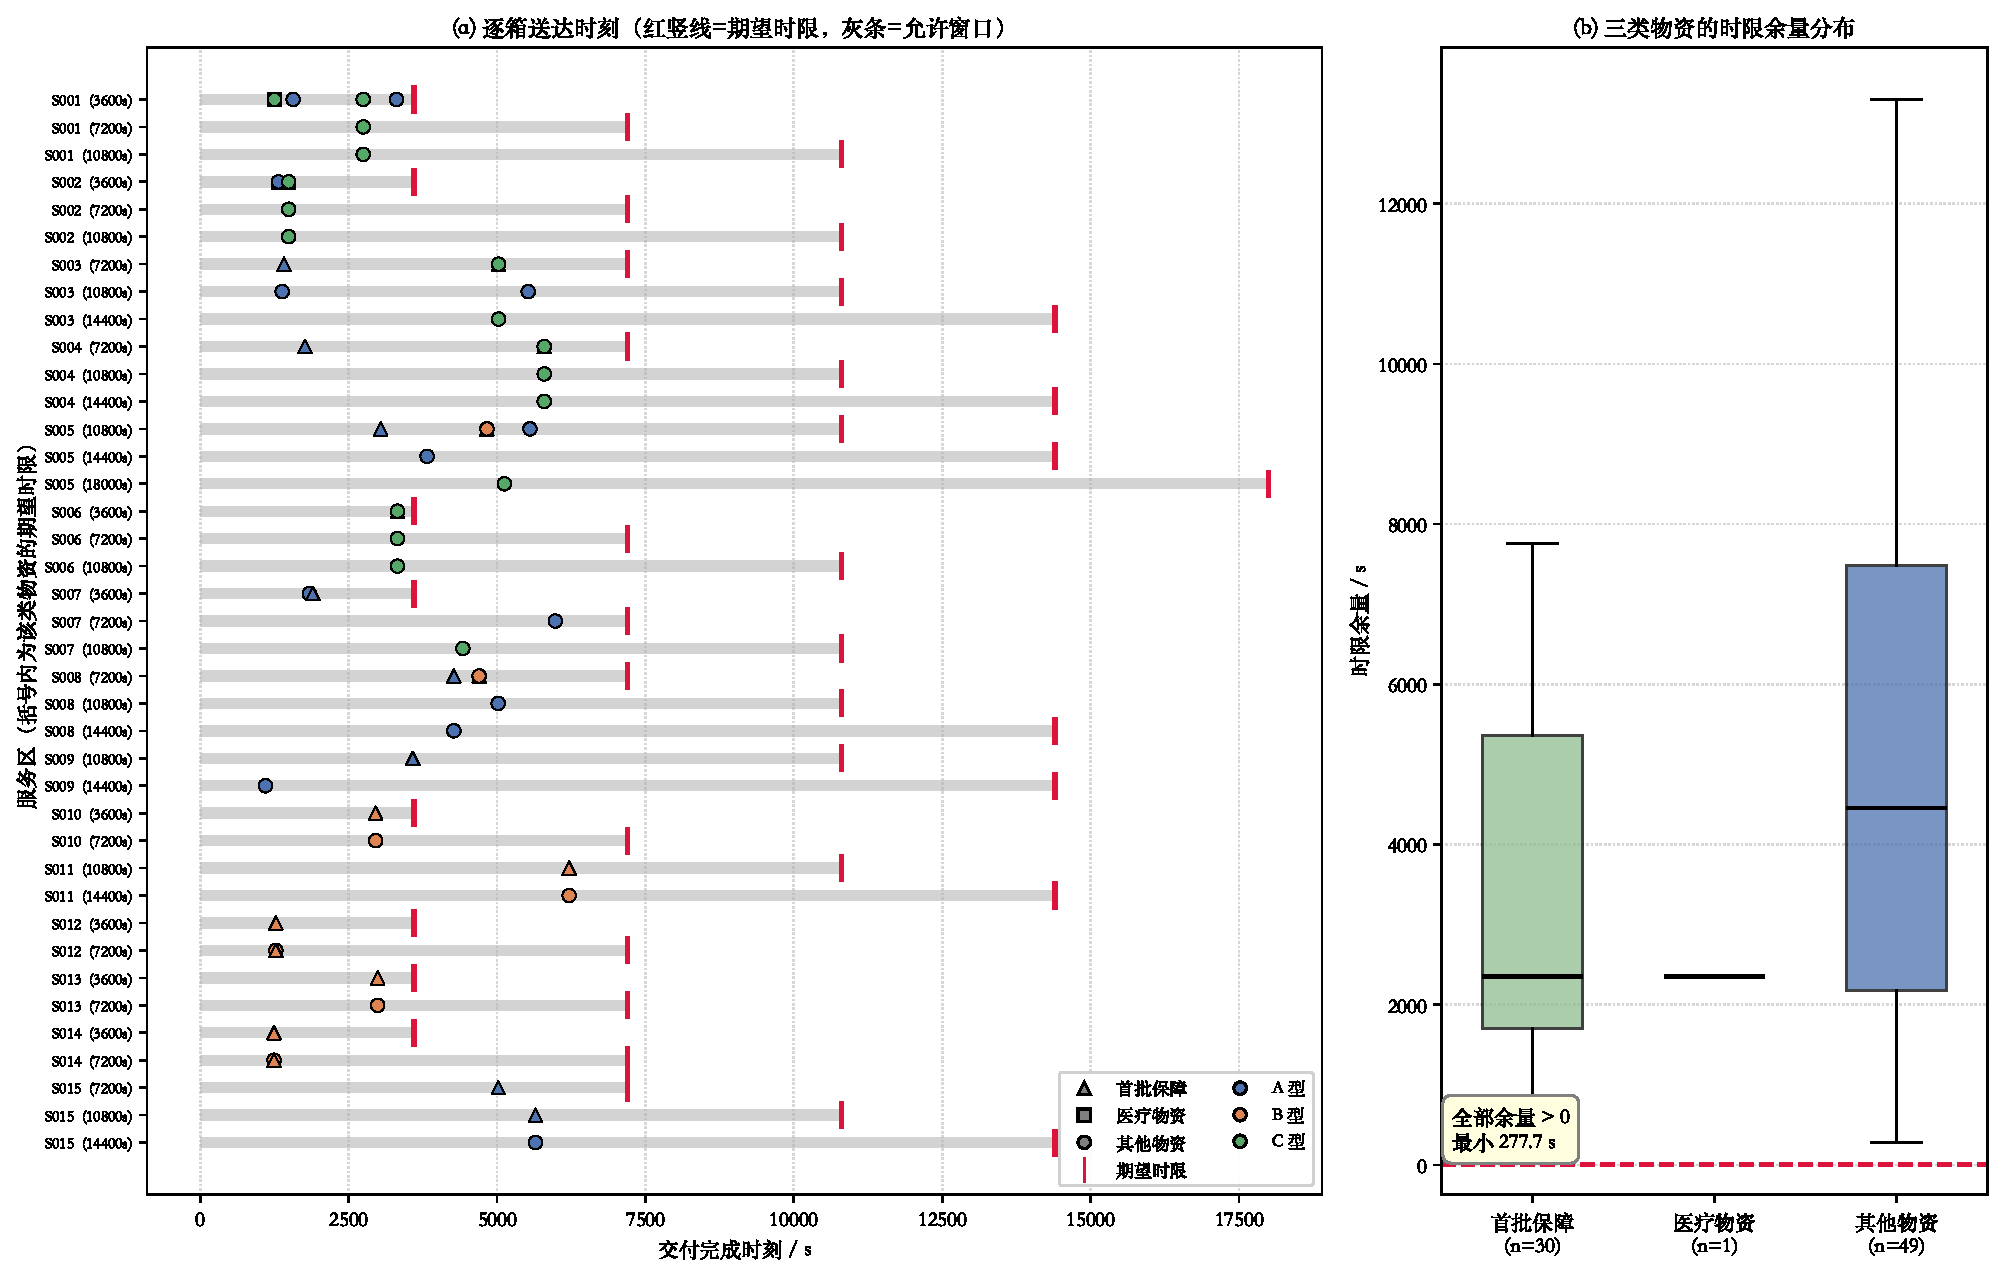
\includegraphics[width=\textwidth]{图/q2_fig6_boxdelivery.pdf}
  \caption{逐箱送达时刻与三类物资的时限余量分布}
  \label{fig:q2-boxdel}
\end{figure}

图~\ref{fig:q2-boxdel}(b) 给出三类物资的时限余量箱线图。
按题目规定的三类时限要求分别核验，结果见表~\ref{tab:q2-timeliness}：

\begin{table}[htbp]
  \centering
  \caption{三类时限要求的分别核验}
  \label{tab:q2-timeliness}
  \begin{tabular}{lccc}
    \toprule
    物资类别 & 箱数 & 时限要求 & 核验结果 \\
    \midrule
    医疗物资     & 16 & 期望送达时间 & 违反 0 箱，最小余量 277.7~s \\
    首批保障货箱 & 30 & 首批截止时间 & 违反 0 箱，最小余量 277.7~s \\
    其他物资     & 49 & 期望送达时间（衡量及时性） & 延误 0 箱，加权延误 $0.0000$ \\
    \midrule
    \textbf{合计} & \textbf{80} & --- & \textbf{按期 80/80} \\
    \bottomrule
  \end{tabular}
\end{table}

其中医疗物资与首批保障货箱为题目\textbf{硬性要求}，均以充足余量满足；
其他物资的期望送达时间虽仅用于"衡量"及时性，本方案亦\textbf{全部达标}，
加权延误为零。

\subsubsection{资源使用情况与可行性检验}

资源使用情况汇总于表~\ref{tab:q2-resuse}。

\begin{table}[htbp]
  \centering
  \caption{无人机与电池资源使用情况}
  \label{tab:q2-resuse}
  \begin{tabular}{lcccc}
    \toprule
    机型 & 架次数 & 使用整机数 & 使用电池组数 & 平均载重利用率 \\
    \midrule
    A & 10 & 4/4 & 6/6 & $19.8/25=79.2\,\%$ \\
    B & 7  & 2/2 & 4/4 & $25.9/30=86.2\,\%$ \\
    C & 6  & 2/2 & 4/4 & $63.2/80=79.0\,\%$ \\
    \midrule
    合计 & 23 & \textbf{8/8} & \textbf{14/14} & --- \\
    \bottomrule
  \end{tabular}
\end{table}

全部 $8$ 架整机与 $14$ 组电池均被调用，无闲置资源，
三类机型的平均载重利用率均在 $79\,\%$ 以上，装载效率较高。
资源占用的时序细节见图~\ref{fig:q2-gantt}：
图 (a) 中任意时刻 A/B/C 型的并发条数分别不超过 $4/2/2$；
图 (b) 中分别不超过 $6/4/4$，均满足式 \eqref{eq:q2-cumul}。
表中的实体编号由第 \ref{subsec:q2-color} 节的区间图贪心着色算法给出。

\subsubsection{解的独立验证}
\label{subsec:q2-verify}

为排除建模与求解过程中的隐性错误，本文编写了\textbf{独立验证程序}，
不依赖候选池索引，仅从解文件自带字段出发重新复算 $16$ 项约束，
包括：货箱覆盖与唯一性、期望延误、硬截止、载重、舱容、电量上限、
整机区间不重叠、电池区间不重叠、机队规模上限、电池组数上限、
以及需求覆盖 $53$ 项匹配等。其中资源不重叠性采用\textbf{区间图贪心着色}
独立重建实体编号分配，与求解器的内部结果完全解耦。

验证结果：\textbf{全部 $16$ 项约束通过}，
$C_{\max}=6568.168$~s，总能耗 $71.3885$~kWh，按期率 $80/80$。

\subsection{结论与讨论}

本问建立了跨区组批与多机协同调度的混合整数规划模型
\eqref{eq:q2-model}，通过装箱、面积、集合分划三类松弛给出了架次数、
完工时刻与总能耗的\textbf{严格理论下界}，并用逻辑型 Benders 分解求得
$N=23$ 时 $C_{\max}=6568.17$~s 的可行解，与面积松弛下界的相对缺口为
$10.5\,\%$，解经 $16$ 项独立验证全部通过。

诊断表明，本问的主导瓶颈是 \textbf{C 型电池的周转能力}而非整机数量：
C 型满充 $3000$~s 使得 $4$ 组电池在 $7$ 架次时无法维持周转。
将机型配比调整为 A$=$10/B$=$7/C$=$6 后，三机型负载极差压缩至 $234$~s。
这一发现对实际运营具有直接指导意义：\textbf{在此类场景下增配电池组的
边际收益高于增配整机}。

\paragraph{尚存的改进空间。}
当前解与下界仍有 $626.83$~s 缺口。该缺口的成因目前\textbf{无法区分}——
可能是解本身仍可改进，也可能是面积松弛过于乐观（实验中已观察到该配比下
多个组合时序不可排）。收紧这一区间需要两方面工作：

\begin{enumerate}
  \item \textbf{强化 Benders 割}。现用的 no-good 割每轮仅排除一个组合，
        泛化能力弱（实测 $22$ 轮仅将 LB 从 $5806$~s 抬升至 $5942$~s），
        宜改为机型计数割或基于冲突核（conflict core）的割；
  \item \textbf{令子问题回灌真实下界}。现子问题仅返回可行/不可行二值信息，
        应改为在放宽窗口上求最小可行 $C_{\max}(S)$ 并回灌至主问题，
        使 LB 得以实质抬升。
\end{enumerate}

若强化后下界越过某阈值，即可\textbf{反向证明该阈值以下不可达}，
这本身亦是具有价值的结论。


\end{document}
